\chapter{Probability Tables}

\vspace{-1.5in}

\section{Normal Distribution}\index{distributions!normal}

Recall from equation (1.1) that the probability density function is
defined by
\begin{equation*}
\mathrm{f}(y)=\frac{1}{\sigma \sqrt{2\pi }}\exp \left(
-\frac{1}{2\sigma ^{2} }\left( y-\mu \right) ^{2}\right)
\end{equation*}
where $\mu$ and $\sigma^2$ are parameters that describe the curve.
In this case, we write $y \sim N(\mu,\sigma^2)$. Straightforward
calculations show that
\begin{equation*}
\mathrm{E}~y = \int_{-\infty}^{\infty} y \mathrm{f}(y) dy =
\int_{-\infty}^{\infty}  y \frac{1}{\sigma \sqrt{2\pi }}\exp \left(
-\frac{1}{2\sigma^2 }\left( y-\mu \right)^2 \right)  dy  = \mu
\end{equation*}
and
\begin{equation*}
\mathrm{Var}~y = \int_{-\infty}^{\infty} (y-\mu)^2 \mathrm{f}(y) dy
= \int_{-\infty}^{\infty} (y-\mu)^2 \frac{1}{\sigma \sqrt{2\pi
}}\exp \left( -\frac{1}{2\sigma^2 }\left( y-\mu \right)^2 \right) dy
= \sigma^2 .
\end{equation*}
Thus, the notation $y \sim N(\mu,\sigma^2)$ is interpreted to mean
the random variable is distributed normally with mean $\mu$ and
variance $\sigma^2$. If $y \sim N(0,1)$, then $y$ is said to be
\emph{standard normal}.

\begin{figure}[htp]
  \begin{center}
    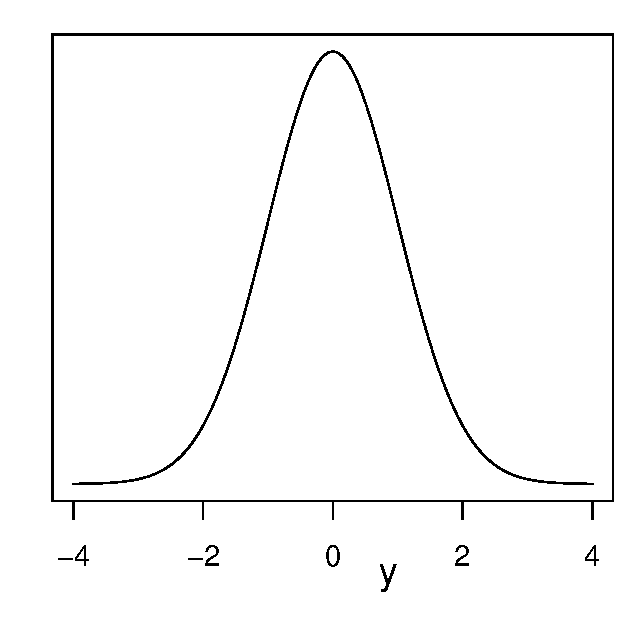
\includegraphics[scale=.6]{Appendices/FAppendNormal.eps}
    \caption{ \small  Standard Normal Probability Density Function.}
  \end{center}
\end{figure}

\begin{table}[h]
\scalefont{0.9} \caption{\label{AP:NormalProbTable} Standard Normal
Distribution Function}
\begin{tabular}{l|rrrrrrrrrr}\hline
         $x$  &          0.0 &        0.1 &        0.2 &        0.3 &        0.4 &        0.5 &        0.6 &        0.7 &        0.8 &        0.9 \\
\hline
         0 &     0.5000 &     0.5398 &     0.5793 &     0.6179 &     0.6554 &     0.6915 &     0.7257 &     0.7580 &     0.7881 &     0.8159 \\
         1 &     0.8413 &     0.8643 &     0.8849 &     0.9032 &     0.9192 &     0.9332 &     0.9452 &     0.9554 &     0.9641 &     0.9713 \\
         2 &     0.9772 &     0.9821 &     0.9861 &     0.9893 &     0.9918 &     0.9938 &     0.9953 &     0.9965 &     0.9974 &     0.9981 \\
3  & 0.9987 & 0.9990 & 0.9993 & 0.9995 & 0.9997 & 0.9998 & 0.9998 &
0.9999& 0.9999&  1.0000 \\
\hline \multicolumn{10}{l}{Probabilities can be found by looking at
the appropriate row for the lead digit } \\
\multicolumn{10}{l}{~~and column for the decimal.
For example, $\Pr ( y \leq 0.1) = 0.5398$.} \\
\hline
\end{tabular}
\scalefont{0.1111}
\end{table}


\newpage
\section{Chi-Square Distribution}\index{distributions!chi-square}

\textbf{Chi-Square Distribution}. Several important distributions
can be linked to the normal distribution. If $y_1, \ldots, y_n$ are
i.i.d. random variables such that each $y_i \sim N(0,1)$, then
$\sum_{i=1}^n y_i^2$ is said to have a \emph{chi-square
distribution} with parameter $n$. More generally, a random variable
$w$ with probability density function
\begin{equation*}
\mathrm{f}(w)=\frac{2^{-k/2}}{\Gamma(k/2)} w^{k/2-1} \exp (-w/2),
~~~~~~w>0
\end{equation*}
is said to have a chi-square with $df=k$ degrees of freedom, written
$w \sim \chi_k^2$. Easy calculations show that for $w \sim
\chi_k^2$, we have E $w = k$ and Var $w = 2 k$. In general, the
degrees of freedom parameter need not be integer, although it is for
the applications of this text.\index{symbols!$\chi_k^2$, chi-square
random variable with $k$ degrees of freedom}

\begin{figure}[htp]
  \begin{center}
    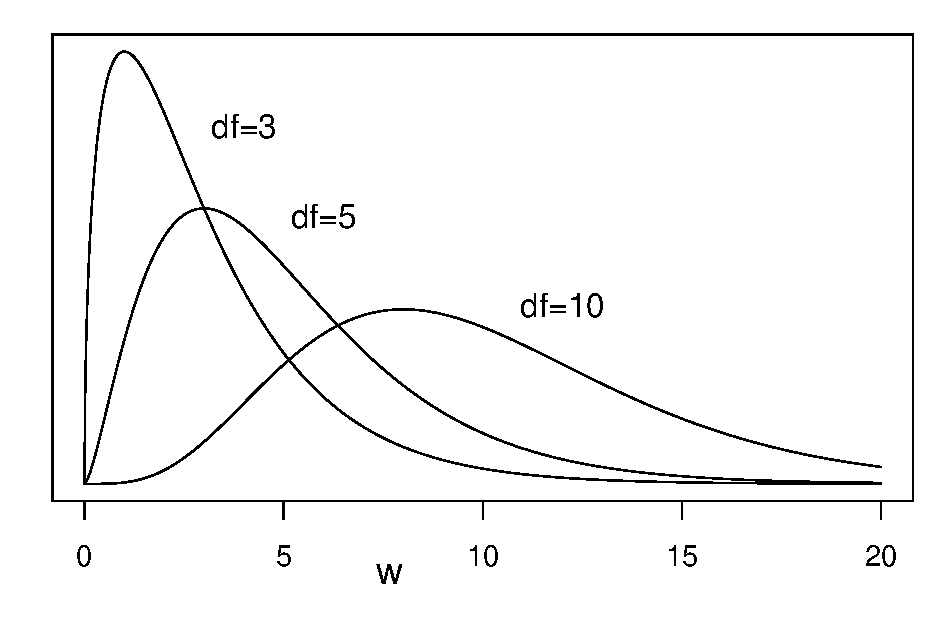
\includegraphics[scale=.6]{Appendices/FAppendChiSq.eps}
    \caption{ \small  Several Chi-Square Probability Density Functions. Shown are curves for $df=3,$
    $df=5$ and $df = 10$. Higher degrees of freedom leads to curves that are less skewed.}
  \end{center}
\end{figure}

\begin{table}[h]
\scalefont{0.9} \caption{\label{AP:ChiSqProbTable} Percentiles from
Several Chi-Square Distributions}
\begin{tabular}{c|rrrrrrrrrr}
\hline   $df$ & \multicolumn{9}{c}{Probabilities} \\
         &        0.6 &        0.7 &        0.8 &        0.9 &       0.95 &      0.975 &       0.99 &      0.995 &     0.9975 &      0.999 \\
\hline
         1 &       0.71 &       1.07 &       1.64 &       2.71 &       3.84 &       5.02 &       6.63 &       7.88 &       9.14 &      10.83 \\
         2 &       1.83 &       2.41 &       3.22 &       4.61 &       5.99 &       7.38 &       9.21 &      10.60 &      11.98 &      13.82 \\
         3 &       2.95 &       3.66 &       4.64 &       6.25 &       7.81 &       9.35 &      11.34 &      12.84 &      14.32 &      16.27 \\
         4 &       4.04 &       4.88 &       5.99 &       7.78 &       9.49 &      11.14 &      13.28 &      14.86 &      16.42 &      18.47 \\
         5 &       5.13 &       6.06 &       7.29 &       9.24 &      11.07 &      12.83 &      15.09 &      16.75 &      18.39 &      20.52 \\
\hline
        10 &      10.47 &      11.78 &      13.44 &      15.99 &      18.31 &      20.48 &      23.21 &      25.19 &      27.11 &      29.59 \\
        15 &      15.73 &      17.32 &      19.31 &      22.31 &      25.00 &      27.49 &      30.58 &      32.80 &      34.95 &      37.70 \\
        20 &      20.95 &      22.77 &      25.04 &      28.41 &      31.41 &      34.17 &      37.57 &      40.00 &      42.34 &      45.31 \\
        25 &      26.14 &      28.17 &      30.68 &      34.38 &      37.65 &      40.65 &      44.31 &      46.93 &      49.44 &      52.62 \\
        30 &      31.32 &      33.53 &      36.25 &      40.26 &      43.77 &      46.98 &      50.89 &      53.67 &      56.33 &      59.70 \\
        35 &      36.47 &      38.86 &      41.78 &      46.06 &      49.80 &      53.20 &      57.34 &      60.27 &      63.08 &      66.62 \\
        40 &      41.62 &      44.16 &      47.27 &      51.81 &      55.76 &      59.34 &      63.69 &      66.77 &      69.70 &      73.40 \\
\hline
        60 &      62.13 &      65.23 &      68.97 &      74.40 &      79.08 &      83.30 &      88.38 &      91.95 &      95.34 &      99.61 \\
       120 &     123.29 &     127.62 &     132.81 &     140.23 &     146.57 &     152.21 &     158.95 &     163.65 &     168.08 &     173.62 \\
\hline
\end{tabular}\scalefont{0.1111}
\end{table}


\newpage
\section{$t$-Distribution}\index{distributions!t-@{$t-$}}
Suppose that $y$ and $w$ are independent with $y \sim N(0,1)$ and $w
\sim \chi_k^2$. Then, the random variable $t = y / \sqrt{w/k}$ is
said to have a $t$-distribution with $df=k$ degrees of freedom. The
probability density function is
\begin{equation*}
\mathrm{f}(t)= \frac{\Gamma \left( k+ \frac{1}{2}
\right)}{\Gamma(k/2)} \left( k \pi \right)^{-1/2} \left( 1 +
\frac{t^2}{k} \right)^{-(k+1/2)}, ~~~~~~-\infty <t<\infty
\end{equation*}
This has mean 0, for $k>1$, and variance $k/(k-2)$ for $k>2$.

\begin{figure}[htp]
  \begin{center}
    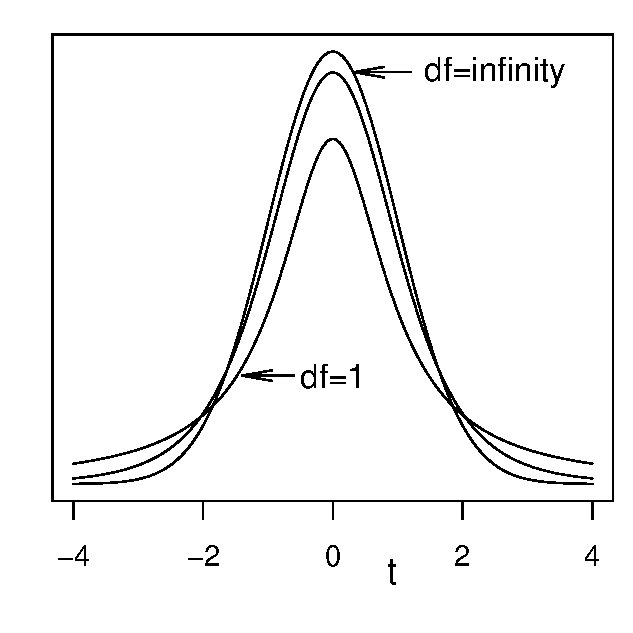
\includegraphics[scale=.6]{Appendices/FAppendt.eps}
    \caption{ \small  Several $t$-Distribution Probability Density Functions.
    The $t$-distribution with $df = \infty$ is the standard normal distribution. Shown are curves for $df=1,$
    $df=5$ (not labeled) and $df = \infty$. A lower $df$ means ``fatter'' tails.}
  \end{center}
\end{figure}


\begin{table}[h]
\scalefont{0.9} \caption{\label{AP:tProbTable} Percentiles from
Several $t-$Distributions}
\begin{tabular}{crrrrrrrrrr}
\hline  $df$ & \multicolumn{9}{c}{Probabilities} \\

           &        0.6 &        0.7 &        0.8 &        0.9 &       0.95 &      0.975 &       0.99 &      0.995 &     0.9975 &      0.999 \\
\hline
         1 &      0.325 &      0.727 &      1.376 &      3.078 &      6.314 &     12.706 &     31.821 &     63.657 &    127.321 &    318.309 \\
         2 &      0.289 &      0.617 &      1.061 &      1.886 &      2.920 &      4.303 &      6.965 &      9.925 &     14.089 &     22.327 \\
         3 &      0.277 &      0.584 &      0.978 &      1.638 &      2.353 &      3.182 &      4.541 &      5.841 &      7.453 &     10.215 \\
         4 &      0.271 &      0.569 &      0.941 &      1.533 &      2.132 &      2.776 &      3.747 &      4.604 &      5.598 &      7.173 \\
         5 &      0.267 &      0.559 &      0.920 &      1.476 &      2.015 &      2.571 &      3.365 &      4.032 &      4.773 &      5.893 \\
\hline
        10 &      0.260 &      0.542 &      0.879 &      1.372 &      1.812 &      2.228 &      2.764 &      3.169 &      3.581 &      4.144 \\
        15 &      0.258 &      0.536 &      0.866 &      1.341 &      1.753 &      2.131 &      2.602 &      2.947 &      3.286 &      3.733 \\
        20 &      0.257 &      0.533 &      0.860 &      1.325 &      1.725 &      2.086 &      2.528 &      2.845 &      3.153 &      3.552 \\
        25 &      0.256 &      0.531 &      0.856 &      1.316 &      1.708 &      2.060 &      2.485 &      2.787 &      3.078 &      3.450 \\
        30 &      0.256 &      0.530 &      0.854 &      1.310 &      1.697 &      2.042 &      2.457 &      2.750 &      3.030 &      3.385 \\
        35 &      0.255 &      0.529 &      0.852 &      1.306 &      1.690 &      2.030 &      2.438 &      2.724 &      2.996 &      3.340 \\
        40 &      0.255 &      0.529 &      0.851 &      1.303 &      1.684 &      2.021 &      2.423 &      2.704 &      2.971 &      3.307 \\
\hline
        60 &      0.254 &      0.527 &      0.848 &      1.296 &      1.671 &      2.000 &      2.390 &      2.660 &      2.915 &      3.232 \\
       120 &      0.254 &      0.526 &      0.845 &      1.289 &      1.658 &      1.980 &      2.358 &      2.617 &      2.860 &      3.160 \\
       $\infty$ &      0.253 &      0.524 &      0.842 &      1.282 &      1.645 &      1.960 &      2.326 &      2.576 &      2.807 &      3.090 \\
\hline
\end{tabular}\scalefont{0.1111}
\end{table}



\newpage
\section{$F$-Distribution}\index{distributions!F-@{$F-$}}

Suppose that $w_1$ and $w_2$ are independent with distributions $w_1
\sim \chi_m^2$ and $w_2 \sim \chi_n^2$. Then, the random variable $F
= (w_1/m) / (w_2/n)$ has an $F$-distribution with parameters
$df_1=m$ and $df_2=n$, respectively. The probability density
function is
\begin{equation*}
\mathrm{f}(y)= \frac{\Gamma \left(\frac{m+n}{2} \right)}
{\Gamma(m/2)\Gamma(n/2)} \left( \frac{m}{n} \right)^{m/2}
\frac{y^{(m-2)/2}} {\left( 1+\frac{m}{n}y \right)^{m+n+2}} ,
~~~~~~y>0
\end{equation*}
This has mean $n/(n-2)$, for $n>2$, and variance
$2n^2(m+n-2)/[m(n-2)^2(n-4)]$ for $n>4$.


\begin{figure}[htp]
  \begin{center}
    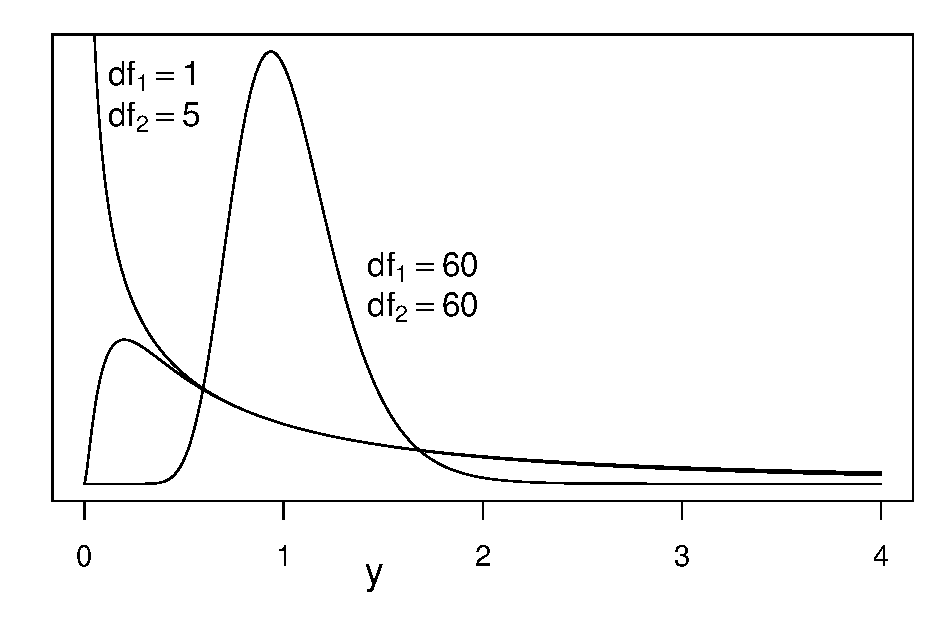
\includegraphics[scale=.6]{Appendices/FAppendF.eps}
    \caption{ \small  Several $F$-Distribution Probability Density Functions.
    Shown are curves for (i) $df_1=1, df_2=5$, (ii)
    $df_1=5, df_2=1$ (not labeled) and (iii) $df_1=60, df_2=60$. As $df_2$ tends to $\infty$,
    the $F$-distribution tends to a chi-square distribution.}
  \end{center}
\end{figure}


\begin{table}[h]
\scalefont{0.9} \caption{\label{AP:FProbTable} Percentiles from
Several $F-$Distributions}
\begin{tabular}{crrrrrrrrr}
\hline  $df_1$ & \multicolumn{9}{c}{$df_2$} \\
           &          1 &          3 &          5 &         10 &         20 &         30 &         40 &         60 &        120 \\
\hline
         1 &     161.45 &      10.13 &       6.61 &       4.96 &       4.35 &       4.17 &       4.08 &       4.00 &       3.92 \\
         2 &     199.50 &       9.55 &       5.79 &       4.10 &       3.49 &       3.32 &       3.23 &       3.15 &       3.07 \\
         3 &     215.71 &       9.28 &       5.41 &       3.71 &       3.10 &       2.92 &       2.84 &       2.76 &       2.68 \\
         4 &     224.58 &       9.12 &       5.19 &       3.48 &       2.87 &       2.69 &       2.61 &       2.53 &       2.45 \\
         5 &     230.16 &       9.01 &       5.05 &       3.33 &       2.71 &       2.53 &       2.45 &       2.37 &       2.29 \\
\hline
        10 &     241.88 &       8.79 &       4.74 &       2.98 &       2.35 &       2.16 &       2.08 &       1.99 &       1.91 \\
        15 &     245.95 &       8.70 &       4.62 &       2.85 &       2.20 &       2.01 &       1.92 &       1.84 &       1.75 \\
        20 &     248.01 &       8.66 &       4.56 &       2.77 &       2.12 &       1.93 &       1.84 &       1.75 &       1.66 \\
        25 &     249.26 &       8.63 &       4.52 &       2.73 &       2.07 &       1.88 &       1.78 &       1.69 &       1.60 \\
        30 &     250.10 &       8.62 &       4.50 &       2.70 &       2.04 &       1.84 &       1.74 &       1.65 &       1.55 \\
        35 &     250.69 &       8.60 &       4.48 &       2.68 &       2.01 &       1.81 &       1.72 &       1.62 &       1.52 \\
        40 &     251.14 &       8.59 &       4.46 &       2.66 &       1.99 &       1.79 &       1.69 &       1.59 &       1.50 \\
\hline
        60 &     252.20 &       8.57 &       4.43 &       2.62 &       1.95 &       1.74 &       1.64 &       1.53 &       1.43 \\
       120 &     253.25 &       8.55 &       4.40 &       2.58 &       1.90 &       1.68 &       1.58 &       1.47 &       1.35 \\
\hline
\end{tabular}\scalefont{0.1111}
\end{table}
